\documentclass{article}
\usepackage{graphicx}

\begin{document}
\section{Question 1}
\setcounter{subsection}{2}
\subsection{}
Time (in seconds) to complete standard training: 1359.3467
Time (in seconds) to complete free adversarial training: 372.3792
\subsection{}
\begin{center}
\begin{tabular}{||c c c||} 
    \hline
    Model/Task & Accuracy & PGD Success rate \\ [0.5ex] 
    \hline\hline
    Standard & 0.9227 & 0.8975 \\ 
    \hline
    Adv.-trained & 0.8235 & 0.3693 \\
    \hline
\end{tabular}
\end{center}
Adversarial training significantly decreases the PGD succees rate, i.e increases robustness with the price of a small decrease in accuracy.
\section{Question 2}
\setcounter{subsection}{1}
\subsection{}
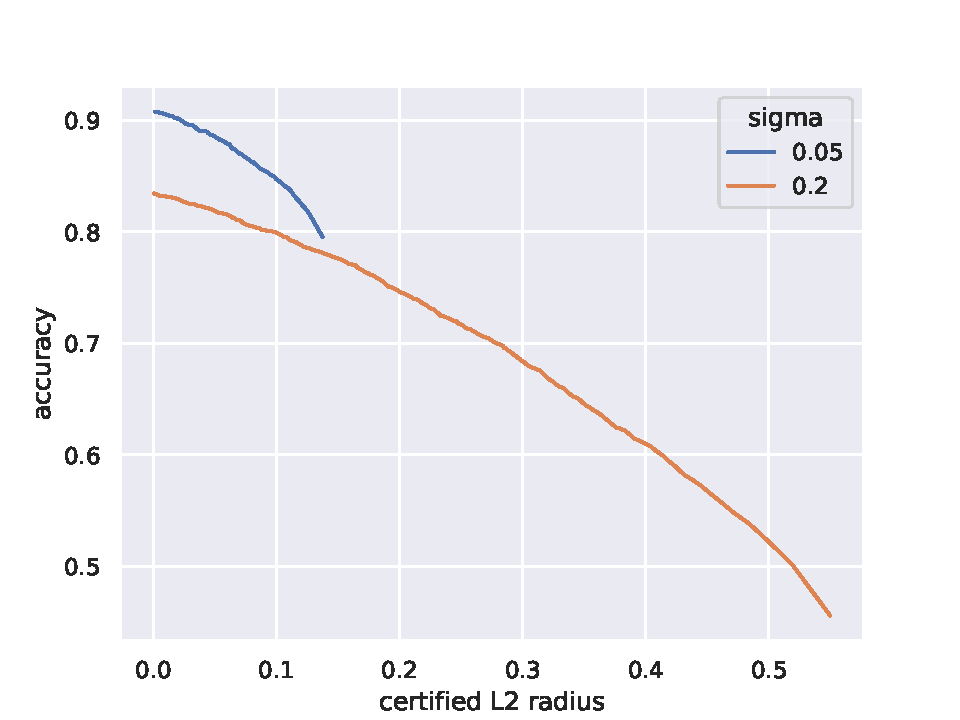
\includegraphics[scale=0.7]{randomized-smoothing-acc-vs-radius.pdf}
\end{document}

